% =============================================================================
% COPYRIGHT AND DISCLAIMER
% =============================================================================
% This file is provided as a convenience template for competition participants.
% By using it, you accept full responsibility for compliance with all applicable
% copyright, licensing, and usage rules of the Association for Computing
% Machinery (ACM) and of any LaTeX packages you load (including, without
% limitation, the "acmart" document class and related ACM materials).
%
% Consult ACM's official publication, template, and copyright policies before
% using this setup for any purpose other than this competition. Do not assume
% that this template may be reused, redistributed, or submitted elsewhere
% without independently verifying ACM's current rules.
%
% Use of the "acmart" class, the "sigconf" option, or ACM-style formatting in
% this template does NOT mean that this report, this competition, its organizers,
% or any resulting PDF is sponsored, endorsed, affiliated with, or published by
% ACM. ACM trademarks and branding remain the property of ACM.
%
% Template packages live in preamble.tex.
% Citations live in main.bib. Edit this file with your paper content.
% =============================================================================
% Organisers' template: https://www.overleaf.com/read/vjztpvrnbrdh (acmart sigconf). Build: latexmk -pdf main.tex
% Figures: fig_pipeline.pdf (scripts/make_figures.py), fig_examples.pdf and fig_distributions.pdf
% (scripts/make_report_figures.py, from the out-of-fold rerun of 12 Nov 2026).

\documentclass[sigconf]{acmart}
% =============================================================================
% Template setup — participants normally do not edit this file.
% Author content belongs in main.tex; citations belong in main.bib.
% \documentclass lives in main.tex so Overleaf does not treat this file as root.
% =============================================================================

% --- Competition / non-ACM-submission friendly rights metadata -------------
\setcopyright{none}
\settopmatter{printacmref=false}
\acmConference[Kaggle Competition]{Filament Segmentation Challenge}{2026}{\href{https://www.kaggle.com/competitions/filament-segmentation-2026}{kaggle.com/competitions/filament-segmentation-2026}}
\acmBooktitle{Competition Report}
\acmDOI{}
\acmISBN{}

% --- Author guidance text --------------------------------------------------
% \guide{...} is gray italic while \guideStyletrue; omitted from the PDF if false.
% Flip the switch in main.tex after % =============================================================================
% Template setup — participants normally do not edit this file.
% Author content belongs in main.tex; citations belong in main.bib.
% \documentclass lives in main.tex so Overleaf does not treat this file as root.
% =============================================================================

% --- Competition / non-ACM-submission friendly rights metadata -------------
\setcopyright{none}
\settopmatter{printacmref=false}
\acmConference[Kaggle Competition]{Filament Segmentation Challenge}{2026}{\href{https://www.kaggle.com/competitions/filament-segmentation-2026}{kaggle.com/competitions/filament-segmentation-2026}}
\acmBooktitle{Competition Report}
\acmDOI{}
\acmISBN{}

% --- Author guidance text --------------------------------------------------
% \guide{...} is gray italic while \guideStyletrue; omitted from the PDF if false.
% Flip the switch in main.tex after % =============================================================================
% Template setup — participants normally do not edit this file.
% Author content belongs in main.tex; citations belong in main.bib.
% \documentclass lives in main.tex so Overleaf does not treat this file as root.
% =============================================================================

% --- Competition / non-ACM-submission friendly rights metadata -------------
\setcopyright{none}
\settopmatter{printacmref=false}
\acmConference[Kaggle Competition]{Filament Segmentation Challenge}{2026}{\href{https://www.kaggle.com/competitions/filament-segmentation-2026}{kaggle.com/competitions/filament-segmentation-2026}}
\acmBooktitle{Competition Report}
\acmDOI{}
\acmISBN{}

% --- Author guidance text --------------------------------------------------
% \guide{...} is gray italic while \guideStyletrue; omitted from the PDF if false.
% Flip the switch in main.tex after \input{preamble}.
%
% Do not use \guide{...} for \email{...}.
\usepackage{xcolor}
\newif\ifguideStyle
\guideStyletrue
\newcommand{\guide}[1]{%
  \ifguideStyle
    {\color{gray!65}\itshape #1}%
  \fi
}

% --- Math ------------------------------------------------------------------
% Do NOT load amssymb (or amsfonts): acmart already loads newtxmath, which
% defines the same symbols (e.g. \Bbbk) and causes a conflict on Overleaf.
% amsmath is already provided by acmart; mathtools extends it.
\usepackage{mathtools}

% --- Figures ---------------------------------------------------------------
% graphicx is already loaded by acmart
\usepackage{subcaption}

% --- Tables ----------------------------------------------------------------
% booktabs is already loaded by acmart
\usepackage{tabularx}
\usepackage{multirow}

% --- Bibliography style is set in main.tex (ACM-Reference-Format) ----------
.
%
% Do not use \guide{...} for \email{...}.
\usepackage{xcolor}
\newif\ifguideStyle
\guideStyletrue
\newcommand{\guide}[1]{%
  \ifguideStyle
    {\color{gray!65}\itshape #1}%
  \fi
}

% --- Math ------------------------------------------------------------------
% Do NOT load amssymb (or amsfonts): acmart already loads newtxmath, which
% defines the same symbols (e.g. \Bbbk) and causes a conflict on Overleaf.
% amsmath is already provided by acmart; mathtools extends it.
\usepackage{mathtools}

% --- Figures ---------------------------------------------------------------
% graphicx is already loaded by acmart
\usepackage{subcaption}

% --- Tables ----------------------------------------------------------------
% booktabs is already loaded by acmart
\usepackage{tabularx}
\usepackage{multirow}

% --- Bibliography style is set in main.tex (ACM-Reference-Format) ----------
.
%
% Do not use \guide{...} for \email{...}.
\usepackage{xcolor}
\newif\ifguideStyle
\guideStyletrue
\newcommand{\guide}[1]{%
  \ifguideStyle
    {\color{gray!65}\itshape #1}%
  \fi
}

% --- Math ------------------------------------------------------------------
% Do NOT load amssymb (or amsfonts): acmart already loads newtxmath, which
% defines the same symbols (e.g. \Bbbk) and causes a conflict on Overleaf.
% amsmath is already provided by acmart; mathtools extends it.
\usepackage{mathtools}

% --- Figures ---------------------------------------------------------------
% graphicx is already loaded by acmart
\usepackage{subcaption}

% --- Tables ----------------------------------------------------------------
% booktabs is already loaded by acmart
\usepackage{tabularx}
\usepackage{multirow}

% --- Bibliography style is set in main.tex (ACM-Reference-Format) ----------

\usepackage{tikz}
\usetikzlibrary{positioning,arrows.meta}

% Guide styling: \guideStyletrue = show gray italic hints; \guideStylefalse = omit them
% \guideStyletrue
\guideStylefalse

\begin{document}

\title{Prompted Recurrent Refinement for Solar Filament Instance Segmentation}  % Replace this with your title
\subtitle{A Solution to the Solar Filament Segmentation Challenge 2026} % DO NOT CHANGE


\author{Ph\d{a}m \DJ\'{u}c C\^{o}ng}
\affiliation{%
  \institution{FPT University}
  \city{Hanoi}
  \country{Vietnam}
}
\email{congpdhe20419@fpt.edu.vn}

\author{L\^{e} Anh \DJ\'{u}c}
\affiliation{%
  \institution{FPT University}
  \city{Hanoi}
  \country{Vietnam}
}
\email{duclahe200666@fpt.edu.vn}

\begin{abstract}
    This report describes our solution to the Solar Filament Segmentation Challenge~2026, a Kaggle competition on automatic segmentation of solar filaments in GONG H-$\alpha$ observations. We use a detect-then-refine
    pipeline whose intermediate outputs (proposals, keep/drop decisions, one mask per candidate) can be inspected
    separately. A frozen DINOv3 ViT-S+/16 with a 0.43\,M-parameter head produces a high-recall filament probability
    map; its low-threshold connected components are filtered by a LightGBM classifier on 32 interpretable features;
    each kept component becomes the \emph{prompt} of a recurrent refiner on DINOv3 ViT-B/16 that segments exactly one
    filament per prompt and predicts whether it exists. On the 707 labelled images, date-disjoint out-of-fold
    evaluation gives Panoptic Quality (PQ) $0.4405$ (95\% bootstrap interval $0.432$--$0.449$), above the $0.34$ of one
    expert annotator scored against another; without test-time augmentation it is $0.436$, against $0.389$ for the
    standard diffusion semantic baseline (DDP) trained on the same folds. The public leaderboard score is $0.39$ ($0.34$ for
    that baseline). Code, weights and notebook:
    \url{https://github.com/Cdshf01230/Solar-Filament-None00000}.
\end{abstract}

\maketitle

\ifguideStyle
\noindent{\color{gray!65}\itshape
Guide mode is on.}
\par\medskip
\fi

\guide{Please limit your report to four (4) pages, excluding the Acknowledgment and References sections. Throughout this document, please follow these considerations:
\begin{itemize}
    \item Do not alter any text that is currently in black color (except for the emails under authors' name).
    \item Replace all gray text with your own.
    \item When you are done with the report, please replace \texttt{\textbackslash guideStyletrue} with \texttt{\textbackslash guideStylefalse}, to remove any gray text. Alternatively, you can remove any text wrapped in \texttt{\textbackslash guide\{\}},
    \item Be as succinct as possible, and only provide details regarding your own work. For example, there is no need to discuss what solar filaments are, or why filament segmentation matters.
    \item If you must, you can add extra sections.
\end{itemize}}


% ==================================== %
%              INTRODUCTION            %
% ==================================== %
\section{Introduction}
    This report goes over the details of our submitted solution to the Solar Filament Segmentation Challenge~2026 \cite{filament-segmentation-2026}. The challenge, launched on July~10,~2026, is organized by the Earth-Space AI Research (ESAIR) Lab\footnote{\href{https://www.esairlab.com/home}{www.esairlab.com/}}. This challenge utilizes the MAGFiLO dataset for evaluation of the segmentation algorithms \cite{ahmadzadeh2024dataset}. The input is a $2048^2$ 8-bit GONG~\cite{gong}
    H$\alpha$ image; the output is one binary mask per filament. Each of the 707 training images (2011--2022) has one to
    three annotation records (411/145/151 images): 1154 records and 8199 masks; 180 images form the test set.
    PQ~\cite{pq} $=\sum_{TP}\mathrm{IoU}/(|TP|+\frac12|FP|+\frac12|FN|)$ with IoU\,$>0.5$ is computed per (image,
    record). We report a strict variant with one-to-one Hungarian~\cite{kuhn} matching, which duplicated masks cannot
    inflate; for our pipeline the organisers' all-pairs rule differs by at most 0.0001 PQ and one TP in every reported
    setting. Annotators disagree substantially: one annotator's masks scored against another's give PQ 0.340 (SQ 0.63)
    on the 296 multi-annotated images. We therefore never merge annotators: every training target and every score uses
    one record, on the full image. Because experts disagree on a filament's extent and identity, our longer-term goal is
    to help people find and correct annotations; we favour stages that can be inspected and used separately over
    combining many model families for a higher automatic score.


% ==================================== %
%              METHODOLOGY             %
% ==================================== %
\section{Methodology}\label{sec:methodology}

\begin{figure*}[t]
\centering
\begin{tikzpicture}[font=\footnotesize, node distance=4.2mm,
  box/.style={draw, rounded corners=2pt, align=center, minimum height=11mm, inner sep=2pt, text width=#1},
  box/.default=25mm, arr/.style={-{Stealth[length=2mm]}, semithick}, note/.style={align=center, text width=27mm, font=\scriptsize\itshape}]
\node[box=15mm, fill=gray!8] (in) {H$\alpha$ image\\$2048^2$, 8-bit};
\node[box=30mm, fill=green!8, right=of in] (s1) {\textbf{1 Proposal}\\frozen DINOv3 ViT-S+/16\\+ 0.43\,M head, 9 tiles of $768^2$};
\node[box=28mm, fill=red!6, right=of s1] (s2) {\textbf{2 Filter}\\components at $p\ge.05$,\\LightGBM on 32 features};
\node[box=29mm, fill=green!8, right=of s2] (s3) {\textbf{3 Refiner}\\DINOv3 ViT-B/16, 3 rounds\\one filament per prompt};
\node[box=28mm, fill=orange!10, right=of s3] (pp) {\textbf{Post-processing}\\presence gate, native\\resampling, anchor\\component, de-duplication};
\node[box=16mm, fill=blue!7, right=of pp] (o) {pixel-disjoint\\instances (RLE)};
\foreach \a/\b in {in/s1, s1/s2, s2/s3, s3/pp, pp/o} \draw[arr] (\a) -- (\b);
\node[note, below=1.5mm of s1] {probability map\\(mean of fold heads)};
\node[note, below=1.5mm of s2] {crops + anchor prompts\\(balanced or recall policy)};
\node[note, below=1.5mm of s3] {mask + presence per prompt\\(5 folds $\times$ 8 D4 transforms)};
\end{tikzpicture}\\[1mm]
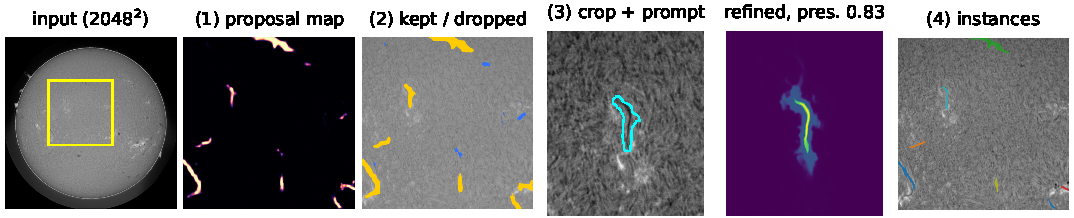
\includegraphics[width=\textwidth]{fig_pipeline.pdf}
\Description{A block diagram of the four steps (proposal, filter, refiner, post-processing) above six image panels
showing a full-disk H-alpha test image, its proposal probability map, kept and dropped components, one refiner crop
with its prompt and refined probability, and the final coloured filament instances.}
\caption{Top: the pipeline; every learned stage yields an output that can be inspected. Bottom: the stages on a test
image (panels 1, 2 and 4 show the $768^2$ window marked on the input). (1) Mean proposal map of the five fold heads;
(2) components at $p\ge.05$ kept by the classifier (yellow) or dropped (blue); (3) one refiner crop with its prompt
(cyan) and its round-3 probability averaged over 5 folds $\times$ 8 transforms; (4) final instances.}
\label{fig:pipeline}
\end{figure*}

\textbf{Data split.} The 707 labelled images are split once into five folds by observation date (seed 42;
141/141/142/141/142 images, 656 days), so near-identical images taken minutes apart never sit on both sides. The
180 test images are used only for the submission. Proposal heads and classifiers are trained on one fold each, and a
labelled image of fold $k$ uses the four that did not see it; refiner $k$ is trained on the other four folds and
predicts fold $k$; at test time all five models of each stage are averaged. Upstream models are reused to build
downstream training inputs, so these are development out-of-fold (OOF) estimates, not fully nested cross-validation.
Proposal threshold, filter threshold and last-epoch checkpoints are fixed; only post-processing was chosen on OOF.

\textbf{Why detect-then-refine.} Instances are not the obstacle in principle: splitting each record's ideal
semantic mask into 8-connected components scores PQ 0.9989. With a predicted mask, however, a faint section splits
one filament and a bridge of false pixels joins two, which is exactly what PQ punishes. On an earlier split (209
training images, 424 held-out) semantic heads of 1.6--2.1\,M parameters on frozen DINOv3~\cite{dinov3} ConvNeXt-B
features reached all-pairs PQ 0.30 (FPN~\cite{fpn}), 0.34 (U-Net~\cite{unet}) and 0.37 (a small variant of the
diffusion head DDP~\cite{ddp}). The best of them, DDP at its standard size (11.6\,M parameters), trained for 20 epochs
on the five folds above, still scores only 0.389 OOF, with about as many false positives as true positives
(Section~\ref{sec:evaluation}). These false positives are confident (median probability 0.95), so no threshold removes
them. We therefore separate \emph{where a filament may be} (cheap, high recall), \emph{which candidates to keep}
(explicit features) and \emph{what exactly this filament is} (one instance per prompt by construction), see
Fig.~\ref{fig:pipeline}.

\textbf{Pre-processing.} The 8-bit image is read in grey, scaled to $[0,1]$, repeated to three channels and normalised
with ImageNet statistics for the backbones; no other filtering is applied.

\textbf{Stage 1: proposal map.} A frozen DINOv3 ViT-S+/16 provides block 3/6/9/12 features; a small FPN-like head with
a half-resolution raw-image branch predicts per-pixel probability on nine $768^2$ tiles blended with a floored Hann
window. It is trained for four epochs with BCE (positive weight 4) + Tversky~\cite{tversky} ($\alpha{=}.2,\beta{=}.8$)
to favour recall. At $p\ge0.05$ the OOF map has pixel recall 0.908 at precision 0.295; ViT-S+ was more precise than a
frozen ConvNeXt-B at equal recall (19.3\% vs 15.4\% at 95\% recall).

\textbf{Stage 2: filter.} The 16,721 OOF components of $p\ge0.05$ (8-connected, $\ge$8\,px) touch 99.3\% of all
filaments. A LightGBM~\cite{lgbm} classifier (250 trees, 15 leaves) on 32 features (shape, probability statistics,
darkness against Gaussian backgrounds, black-hat responses, thickness, elongation, context contrast) keeps components
with mean score $\ge0.5$, and each kept component gives a crop (bounding box + 128\,px). The default
\emph{balanced} policy keeps 5493 components, and 95.1\% of the filaments intersect a retained crop. A released
\emph{recall-oriented} policy (positive class weight $\times48$) keeps 9411 (99.5\%) for reviewing candidates; the
refiner was trained on balanced crops and its PQ on recall crops has not been measured.

\textbf{Stage 3: prompted recurrent refiner.} The crop is letterboxed to $512^2$ with five stem channels: image,
proposal probability, anchor (the component), signed distance to it and current mask; letterbox validity is separate.
A five-level convolutional stem is added at stride 16 to projected DINOv3 ViT-B/16 features (blocks 1--8 frozen,
9--12 fine-tuned with layer-wise LR decay 0.65 and drop path~\cite{droppath} 0.1), followed by four global
self-attention blocks with a round embedding, so the two ends of a long filament can inform each other, and a U-Net
decoder. Three recurrent rounds feed the previous mask back. A presence head predicts $\mathrm{logit}$(ML score) plus a
learned residual. The target is, per record, the filament overlapping the anchor most; prompts are the anchor (40\%),
a corrupted target (30\%, eight corruption types), the model's own rollout (20\%) or empty (10\%). The loss sums BCE +
Lov\'asz hinge~\cite{lovasz}, presence BCE, an empty-crop term and Skeleton Recall~\cite{skel} over all rounds, with
D4, photometric and scale augmentation. Each fold model trains 30 epochs and the last checkpoint is used
(34,820,802 trainable parameters).

\textbf{Post-processing.} Prompts with presence $<0.5$ are dropped. The round-3 probability is resampled bilinearly to
native size and thresholded at $p>0.5$; the component overlapping the anchor most is kept ($\ge128$\,px). Candidates
are accepted greedily by presence, skipping those with IoU $>0.5$ to an accepted one and removing already-taken pixels
(kept if $\ge128$ remain), so instances are pixel-disjoint. At test time the five fold refiners and eight dihedral
transforms are averaged (40 passes per crop).

% ==================================== %
%              EVALUATION              %
% ==================================== %
\section{Evaluation}\label{sec:evaluation}

\textbf{Strategy.} All scores are OOF on the 707 labelled images, computed per original annotation record on the
full image and counting filaments lost by any stage as false negatives; TP, FP, FN and the IoU sum are pooled over
the 1154 records before PQ is computed. Uncertainty is given by a bootstrap over images (2000 resamples) and by the
spread of the five folds.

\begin{table}[t]
\caption{OOF results (707 images, 1154 records, 8199 GT; strict matching). 95\% intervals: bootstrap over images.}
\label{tab:main}
\centering
\footnotesize
\setlength{\tabcolsep}{3.5pt}
\begin{tabular}{@{}lccrrr@{}}
\toprule
Setting & PQ & SQ & TP & FP & FN \\
\midrule
threshold at 512, nearest upsampling & .4227 & .669 & 4993 & 2621 & 3206 \\
+ bilinear native resampling & .4363 & .681 & 5065 & 2549 & 3134 \\
+ D4 TTA (\textbf{submitted}) & \textbf{.4405} & .683 & 5100 & 2512 & 3099 \\
\quad 95\% bootstrap interval & \multicolumn{5}{l}{[.432, .449]} \\
\quad mean $\pm$ SD of the 5 folds & \multicolumn{5}{l}{.441 $\pm$ .010 (range .430--.452)} \\
\quad rerun of the released code (L4) & .4405 & .683 & 5095 & 2498 & 3104 \\
LOFO post-processing selection & .4395 & .683 & & & \\
\midrule
DDP baseline, same folds, no TTA & .3886 & .674 & 5557 & 5509 & 2642 \\
annotator vs.\ annotator (all-pairs) & .340 & .63 & & & \\
\bottomrule
\end{tabular}
\end{table}

\begin{figure*}[t]
\centering
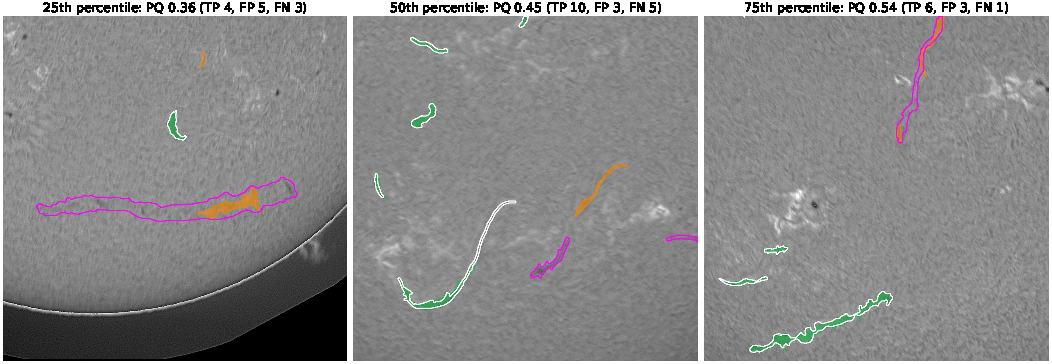
\includegraphics[width=\textwidth]{fig_examples.pdf}
\Description{Three zoomed windows of labelled H-alpha images with predicted filament masks filled in green or orange
and annotated filaments outlined in white or magenta.}
\caption{OOF predictions on the labelled images ranked at the 25th, 50th and 75th percentile of per-image PQ (among
single-annotator images with at least six filaments; $896^2$ windows). Green: prediction matched one-to-one with IoU
$>0.5$; orange: unmatched prediction; white outline: matched annotation; magenta outline: missed annotation. The
typical error is a filament painted only in part (orange inside a magenta outline).}
\label{fig:examples}
\end{figure*}

\begin{figure*}[t]
\centering
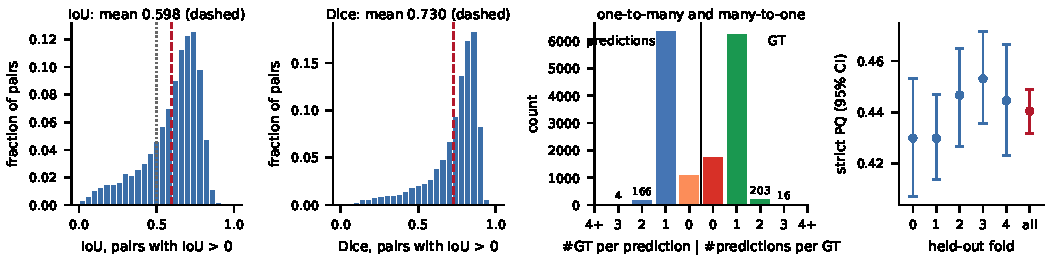
\includegraphics[width=\textwidth]{fig_distributions.pdf}
\Description{Four plots: histograms of IoU and Dice for overlapping ground-truth and prediction pairs, a two-sided bar
chart of how many predictions overlap each ground-truth filament and vice versa, and per-fold PQ with error bars.}
\caption{The organisers' rubric statistics on the OOF rerun (1154 records). Left to right: IoU and Dice of every
(annotation, prediction) pair that overlaps (IoU $>0$); number of annotations each prediction overlaps and number
of predictions each annotation overlaps (degree $\ge2$: many-to-one and one-to-many); strict PQ per held-out fold
and pooled, with 95\% bootstrap intervals over images.}
\label{fig:distributions}
\end{figure*}

\textbf{Results.} Table~\ref{tab:main} gives the main scores. Resampling probabilities instead of masks improved 24/24
earlier model--fold pairs; test-time augmentation adds 0.004. Leave-one-fold-out (LOFO) selection among 11 stored
post-processing settings gives 0.4395, a check of setting selection only. The organisers' self-evaluation code on our
OOF predictions returns 0.440524, equal to our all-pairs scorer. One-change-at-a-time ablations on a single split
showed the largest gains from D4 augmentation (+0.039), the ML-anchored presence (+0.009) and layer-wise LR decay with
drop path (+0.007). The public leaderboard score is 0.39 (about half of the test images).

\textbf{Dice, IoU and one-to-many / many-to-one.} Fig.~\ref{fig:distributions} gives the statistics of the organisers'
self-evaluation notebook, computed per record on the OOF rerun of Section~\ref{sec:code}. The 6696 overlapping pairs
have mean IoU 0.598 and mean Dice 0.730; the 5095 strict true positives have mean IoU 0.683 and mean Dice 0.808. Of
the 8199 annotated filaments, 76\% overlap exactly one prediction, 21\% none and 219 (2.7\%) two or more
(one-to-many); 170 of 7593 (prediction, record) pairs (2.2\%) overlap two or more filaments (many-to-one). The Dice
of the union of the predicted masks against the union of a record's masks is 0.664 on average (0.690 pooled).
Fig.~\ref{fig:examples} shows predictions on images of low, median and high PQ.

\textbf{Efficiency.} On one NVIDIA L4 the released \texttt{predict.py} processes the 180 test images in 84\,min
(28\,s per image, models loaded once): stages 1--2 take 5.1\,s per image (five proposal heads on one frozen backbone,
components, features and LightGBM) and stage 3 takes 0.57\,s per crop for each fold refiner with eight transforms
(7.9 crops per image, five refiners). Stage 3 is 80\% of the time; without TTA it is eight times cheaper and loses
0.004 PQ (Table~\ref{tab:main}). Trainable parameters are 0.43\,M per proposal head, 250 trees per classifier and
34.8\,M per refiner, on frozen DINOv3 ViT-S+/16 (28.7\,M) and ViT-B/16 (85.7\,M) backbones.

\textbf{Semantic baseline.} The standard DDP semantic head (11.6\,M parameters, frozen ConvNeXt-B, threshold 0.5,
8-connected components), trained for 20 epochs on the same five folds with a cosine learning-rate decay that ends at
29\% of its peak, scores 0.3886 OOF (choosing its epoch on the other four folds: 0.3924), against 0.4363 for our
pipeline without TTA, with
more than twice as many false positives (5509 vs 2549); its five-fold ensemble scores 0.34 on the public leaderboard
against our 0.39.

\textbf{Error analysis.} The 3099 false negatives fall into disjoint classes: 1329 lie inside a crop but are touched by
no prediction (514 only in crop padding), 558 are incomplete masks, 402 are lost before the refiner, 332 are too wide,
219 merged with a neighbour, 146 misaligned, 82 split and 31 taken by another match or by the presence gate. Across
classes, 481 share an anchor with another filament and are never a crop target, since a prompt yields one instance.
For incomplete masks 77\% have a single anchor that already covers a median 81\% of the filament: the refiner sees the
missing part but does not paint it. Removing every false positive on annotation background would raise PQ only to
0.473; background means unmatched to that record, not verified physical absence.

\textbf{Strengths, weaknesses and improvements.} Every stage has an output a person can inspect, each instance comes
from an explicit prompt, and instances never overlap, so a filament cannot be counted twice. Its limits are
the recall cost of filtering (a filament outside every crop cannot be recovered), incomplete masks and one output per
prompt. Re-prompting on the part of an anchor the first mask does not explain finds up to 164 of the 506
never-targeted filaments, but at 14\% precision, so the best zero-shot variant (0.4409) is within noise. A trained
second output per prompt, mask completion and a refiner trained on recall-policy crops are the next steps. Support
for annotation is an intended use that has not yet been validated in a user study.

% ==================================== %
%       CODE AND REPRODUCIBILITY       %
% ==================================== %
\section{Code and reproducibility}\label{sec:code}
The repository contains the inference package (one module per stage, all constants in one file), a notebook that
loads the weights from the repository, runs every stage with visualisations, reproduces the submission and evaluates
OOF, pinned requirements, all weights (1.1\,GB; refiner files store only the decoder and the four fine-tuned blocks,
the rest verified bit-identical to the public DINOv3 weights) and the training code of every stage. On 12 November
2026 we downloaded the code and weights from the public Hugging Face copy (identical to GitHub), installed the pinned
requirements on a Colab L4 and reran everything: the 180-image test CSV was byte-identical to the submitted one, and
the OOF run on all 707 images gave PQ 0.440507 against 0.440463 recorded (555 images identical; the others differ
slightly because stage-1 maps are recomputed instead of read from storage). Fresh training from scratch has not been
repeated. Mirror: \url{https://huggingface.co/None00000/Solar-Filament-None00000}.

% ==================================== %
%            ACKNOWLEDGMENT            %
% ==================================== %
\section{Acknowledgment}\label{sec:acknowledgment}
    % Do not change
    The organization of the Filament Segmentation Challenge 2026 is partially supported by the U.S. National Science Foundation (NSF) under Grant No. 2209912 and 2433781, directorate for Computer and Information Science and Engineering (CSE), and Office of Advanced Cyberinfrastructure (OAC), and Grant No. 2511630, AST Division Of Astronomical Sciences and MPS Directorate for Mathematical and Physical Sciences.

    The Filament Segmentation Challenge 2026 is sponsored by the U.S. National Science Foundation (NSF) National Solar Observatory (NSO).

    This work utilizes GONG data obtained by the NSO Integrated Synoptic Program, managed by the National Solar Observatory, which is operated by the Association of Universities for Research in Astronomy (AURA), Inc. under a cooperative agreement with the National Science Foundation and with contribution from the National Oceanic and Atmospheric Administration. The GONG network of instruments is hosted by the Big Bear Solar Observatory, High Altitude Observatory, Learmonth Solar Observatory, Udaipur Solar Observatory, Instituto de Astrofísica de Canarias, and Cerro Tololo Interamerican Observatory.

\bibliographystyle{ACM-Reference-Format}
\bibliography{main}

\end{document}
